\section{Analysis}

\begin{frame}
\frametitle{Time Complexity}

Perl, Ruby, Java, Python, \dots 등이 제공하는 정규 표현식 라이브러리들은 
경우에 따라 프로그램 실행 시간이 입력의 
크기에 지수적으로 비례해서 증가하는 문제를 일을킬 수 있다. 

Figure \ref{fig:graph}의 두 그래프는 입력의 길이 $n$과 수행 시간 과의 
상관 관계를 보여 준다. 좌측은 시간 단위가 seconds이고 우측은 
microsenconds인 점을 주목하라.

\begin{figure}
\begin{columns}[b]
    \column{.45\paperwidth}
        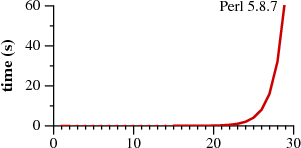
\includegraphics[width=.35\paperwidth]{grep3p.png}
    \column{.45\paperwidth}
        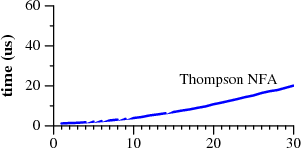
\includegraphics[width=.35\paperwidth]{grep4p.png}
\end{columns}
\[
    \rmatch{a}{a?a},  \rmatch{aa}{a?a?aa}, \dots 
\]
\caption{Time to match ``$\mbtt{a?}^n\mbtt{a}^n$'' against
``$\mbtt{a}^n$''.\footnote{\href{http://swtch.com/~rsc/regexp/regexp1.html}{``Regular Expression
    Matching Can Be Simple And Fast''}. Russ Cox}}
\label{fig:graph}
\end{figure}


\end{frame}

\begin{frame}[shrink]
\frametitle{Backtracking}

Figure \ref{fig:graph}의 결과는 backtracking의 존재 여부에 따른 것이다.
오늘날 거의 대부분의 프로그래밍 언어들은 속도 보다는 backreference 등의 기능을 
제공하기 위해  NFA 기반의 정규 표현식 구현을 채택하고
있다.

\begin{block}{Example}
``$\texttt{ab}^{*}\texttt{b}$'' matches ``$\texttt{abb}$''.
\[
  \begin{array}{lllllllllll}
    &   &             &         &             &\stackrel{4}{\nearrow} &
    \rmatch{\e}{b^{*}b}&\stackrel{7}{\ra}& \F &  \\
    \rmatch{abb}{ab^{*}b} &\stackrel{1}{\ra}& \rmatch{bb}{b^{*}b} & \stackrel{2}{\ra}
    & \rmatch{b}{b^{*}b} &\stackrel{5}{\ra}     & \rmatch{\e}{\e}
    &\stackrel{8}{\ra}& \T &  \\
    &   &             & \stackrel{3}{\searrow} & \rmatch{b}{\e}
    &\stackrel{6}{\ra}     & \F  & &  & &   
  \end{array}
\]
1,2,5,8의 순서로 프로그램이 실행된다면 단번에 
정규표현식 ``$\texttt{ab}^{*}\texttt{b}$''이 문자열  ``$\texttt{abb}$''과
match된다는 것을 알 수 있다. 하지만 NFA 기반 정규 표현식 matcher는 6이나 
7까지 실행을 하는 경우가 생기므로 수행 시간이 길어 질 수 있다.
\end{block}

참고로 grep, awk 등의 command line 도구 들은 DFA를 채택하고 있다.

\end{frame}

\begin{frame}
\frametitle{수행 시간이 입력의 크기에 선형적으로 비례하는 Regular Expression Matcher}

실제 정규 표현식의 적용에서 backreference 등 유연하고 
다양한 feature가 필요 없는 경우가 많다.
여기서 speed, reliability 등이 보장되는 regular expression matcher의 
필요성이 대두 된다.

개발자에게 하나의 선택권만 주는 것 보다는 하나의 옵션을 더 제공함으로써
요구사항에 맞는 기능을 개발할 수 있게 할 필요가 있다.

\end{frame}
